\index{global optimization}
\index{complexity analysis}
\chapter{Global Optimization}
\newthought{And then there were many.} 


% ==============================================================================================
% INTRODUCTION BLOCK

\section{The Why}
\index{global optimization} \index{local minima}

\newthought{In the previous chapter,} we developed Newton's method and gradient descent for finding roots.
The methods we learned about are local methods: They converge to whatever solution is nearby.
But what if the nearby solution is bad? Or if another solution is much better but farther away?

\newthought{Time to do away with oversimplifications.} In this chapter, we will:
\begin{itemize}
    \item Learn about Shekel's foxholes, a classic test function for global optimization
    \item Shortly show, how we can formulate an optimization problem as a root-finding problem.
    \item Introduce strategies for finding global minima
\end{itemize}


\marginnote{\newthought{Visualization of neural network loss landscapes} Li et al. (2018) shows the complex terrain of neural network optimization. Different initializations lead to different final solutions.}

\newthought{In machine learning and especially deep learning,} understanding multi-dimensional and global optimization is crucial for training 
large models effectively, and to make them converge, and actually learn something useful. Neural network loss 
landscapes \cite{VisualizeLandscape} are highly non-convex, do have flat regions, and contain many local minima, 
making optimization challenging.






\newpage
\subsection{Hands On Experience}
\index{hands-on} \index{multimodal}

\newthought{Shekel's foxholes} is a classic test function for global optimization with controlled multimodality. In 1D, it takes the simple form:

\begin{equation}
    f(x) = -\sum_{i=1}^{m} \frac{c_i}{(x - a_i)^2 + r_i}
\end{equation}

where $a_i$ are the ``foxhole'' locations, $c_i$ controls the depth of each hole, and $r_i$ controls the width. 
By adjusting these parameters, we can create a landscape with multiple local minima and one global minimum, making it an ideal playground for testing optimization algorithms.
Consider a specific example with three foxholes:



\begin{figure}[h]
    \centering
    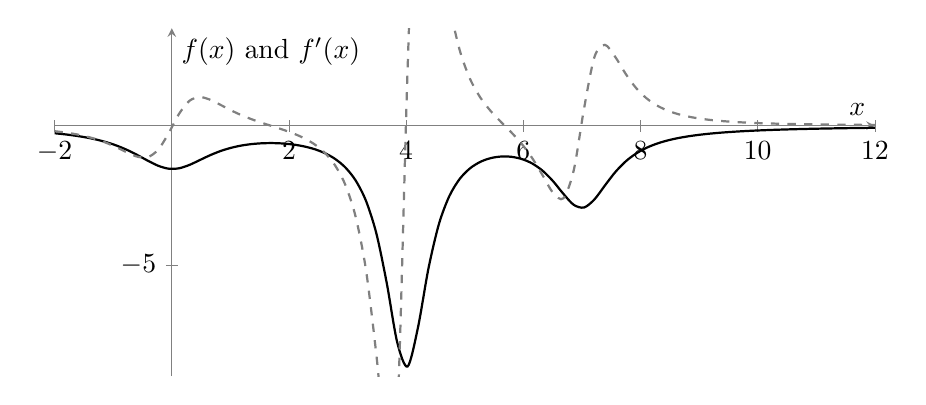
\begin{tikzpicture}
        \begin{axis}[
            width=12cm,
            height=6cm,
            axis x line=middle,
            axis y line=middle,
            xlabel={$x$},
            ylabel={$f(x)$ and $f'(x)$},
            domain=-2:12,
            samples=80,
            ymin=-9, ymax=3.5,
            xmin=-2, xmax=12,
            tick style={gray},
            label style={black},
            axis line style={gray},
        ]
        \addplot[
            black,
            thick,
            smooth,
        ] {-1/((x-0)^2 + 0.7) - 1.7/((x-4)^2 + 0.2) - 1.1/((x-7)^2 + 0.4)};
        
        \addplot[
            gray,
            dashed,
            thick,
            smooth,
        ] {2*(x-0)/((x-0)^2 + 0.7)^2 + 3.4*(x-4)/((x-4)^2 + 0.2)^2 + 2.2*(x-7)/((x-7)^2 + 0.4)^2};
                
        \end{axis}
    \end{tikzpicture}
    \caption{A 1D Shekel's foxholes function (black) with three local minima and its derivative (gray dashed). The function has valleys at $x = 0, 4, 7$, with the deepest (global minimum) at $x = 4$. The derivative (dashed line) crosses zero at each minimum.}
    \label{fig:shekel_foxholes_1d}
\end{figure}


\marginnote{\newthought{The derivative}, illustrated as the dashed line is the answer to formulating optimization as root finding. The minima of $f(x)$ correspond to the roots of $f'(x)$.}


\begin{equation*}
    f(x) = -\frac{1}{(x-0)^2 + 0.7} - \frac{1.7}{(x-4)^2 + 0.2} - \frac{1.1}{(x-7)^2 + 0.4}
\end{equation*}

\newthought{The global minimum} is at $x = 4$. The other two minima at $x = 0$ and $x = 7$ are local minima, respectively. 
This information is of course not available to us when we run an optimization algorithm. We only see the function values and gradients at the points we evaluate. But the knowledge 
comes in handy for exploring the behavior of optimization methods.



\newthought{The sensitivity to initial conditions} of $x_0$ is something you already experienced. 
If we start Newton's method near $x = 0$ or $x = 7$, we'll converge to a local minimum, not the global one at $x = 4$. 


\newthought{Let's apply Newton's method} to our 1D Shekel function\cite{shekel1971test} from different starting points and observe where the method converges.
Let's show it for one starting point, try another one yourself, and then we will discuss the general behavior.

\newthought{From $x_0 = 7.2$:} Newton's method converges to the local minimum at $x \approx 7$. 
To apply Newton's method to optimization, we solve the root finding problem on $f'(x) = 0$, to reformulate the optimization problem.
The Newton update becomes:
\begin{equation}
    x_{n+1} = x_n - \frac{f'(x_n)}{f''(x_n)}
\end{equation}

\begin{figure}[h]
    \centering
    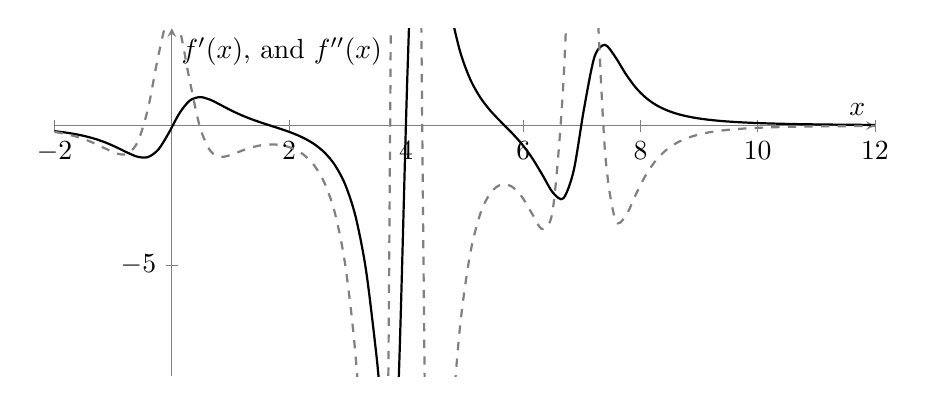
\begin{tikzpicture}
        \begin{axis}[
            width=12cm,
            height=6cm,
            axis x line=middle,
            axis y line=middle,
            xlabel={$x$},
            ylabel={$f'(x)$, and $f''(x)$},
            domain=-2:12,
            samples=80,
            ymin=-9, ymax=3.5,
            xmin=-2, xmax=12,
            tick style={gray},
            label style={black},
            axis line style={gray},
        ]
        \addplot[
            black,
            thick,
            smooth,
        ] {2*(x-0)/((x-0)^2 + 0.7)^2 + 3.4*(x-4)/((x-4)^2 + 0.2)^2 + 2.2*(x-7)/((x-7)^2 + 0.4)^2};
        
        \addplot[
            gray,
            dashed,
            thick,
            smooth,
        ] {2*(0.7 - 3*(x-0)^2)/((x-0)^2 + 0.7)^3 + 3.4*(0.2 - 3*(x-4)^2)/((x-4)^2 + 0.2)^3 + 2.2*(0.4 - 3*(x-7)^2)/((x-7)^2 + 0.4)^3};
                
        \end{axis}
    \end{tikzpicture}
    \caption{A 1D Shekel's foxholes function's first derivative (black), and second derivative (gray dashed). The function has valleys at $x = 0, 4, 7$, with the deepest (global minimum) at $x = 4$. The first derivative crosses zero at each minimum, and the second derivative is positive at minima (confirming local curvature).}
    \label{fig:shekel_foxholes_derivatives}
\end{figure}

The derivatives simplify to:
\begin{align*}
    f'(x) &= \frac{2x}{(x^2 + 0.7)^2} + \frac{3.4(x-4)}{((x-4)^2 + 0.2)^2} + \frac{2.2(x-7)}{((x-7)^2 + 0.4)^2} \\[0.5em]
    f'(7.2) &\approx 0.005 + 0.100 + 2.27 \\
    &= 2.38 \\
    \\
    f''(x) &= \frac{2(0.7 - 3x^2)}{(x^2 + 0.7)^3} + \frac{3.4(0.2 - 3(x-4)^2)}{((x-4)^2 + 0.2)^3} + \frac{2.2(0.4 - 3(x-7)^2)}{((x-7)^2 + 0.4)^3}\\[0.5em]
    f''(7.2) &\approx -0.002 - 0.091 + 7.23 \\
    &= 7.14 \\
    \\  
    x_1 &= 7.2 - \frac{2.38}{7.14} \\
    &\approx 6.87 \\
    \\
    x_2 &\approx 7.02 \\
    x_3 &\approx 7.00
\end{align*}

\vspace{1.5em}
See how root finding methods can be used for optimization by applying them to the derivative of the function.
The derivative $f'(x)$ is zero at extrema, so at this point we find minima or maxima.

\marginnote{\newthought{Local minima notation:} The asterisk (*) is conventionally reserved for global optima. 
To distinguish local from global minima, consider alternative notation like $x^{\circ}$ (x-circle) or $x_i$ for the $i$-th local minimum.}

Here, we were unlucky, and the method is attracted to the nearby foxhole at $x^{\circ} \approx 7$.


\newthought{The fundamental problem however is} that local optimization only guarantees finding a nearby extrema. 
Even with convergence guarantees, we would have got lucky starting from $x_0 = 3$, but from $x_0 = -2$ or $x_0 = 8$, we miss the global minima. 
Enough motivation for the global optimization strategies we'll discuss next.



\vspace{2.5em}
\newthought{The Learning Objectives} of this chapter aim at providing you with the abilities to:
\begin{itemize}
    \item Explain why local methods cannot guarantee finding global minima
    \item Apply strategies for finding global extrema
    \item Understand how gradient descent helps to direct optimization towards minima
\end{itemize}











% ==============================================================================================
% MAIN THEORY BLOCK

\newpage

%% ---- TOPIC 1: Global Optimization Strategies ----

\section{Global Optimization Strategies}
\index{local optimization} \index{global optimization}

Let us formalize local and global extrema.

\newthought{Local optimization} finds a nearby minimum:
\begin{equation}
    \mathbf{x}^* = \arg\min_{\mathbf{x} \in \mathcal{N}(\mathbf{x}_0)} f(\mathbf{x})
\end{equation}
where $\mathcal{N}(\mathbf{x}_0)$ is some neighborhood of the starting point.

\marginnote{\newthought{$\mathcal{N}$ is a set} of points around $\mathbf{x}_0$. For example, $\mathcal{N}(\mathbf{x}_0) = \{\mathbf{x} : \|\mathbf{x} - \mathbf{x}_0\| < \epsilon\}$ for some radius $\epsilon$.}

\newthought{Global optimization} finds the best minimum:
\begin{equation}
    \mathbf{x}^* = \arg\min_{\mathbf{x} \in \Omega} f(\mathbf{x})
\end{equation}
where $\Omega$ is the entire search domain. It is easy to see how the search domain can be inifinitely large. 

\marginnote{\newthought{Convex vs.\ non-convex:} A function $f$ is \emph{convex} if $f(\lambda x + (1-\lambda)y) \leq \lambda f(x) + (1-\lambda)f(y)$ for all $\lambda \in [0,1]$. For convex functions, every local minimum is the global minimum---local methods suffice. Non-convex functions (like Shekel's foxholes or neural network loss surfaces) are the hard case.}

\newthought{Convexity is the dividing line.} For convex problems, any local method will find the global optimum. The difficulty arises in non-convex optimization, 
where the landscape contains multiple local minima, saddle points, and plateaus.


\index{random restarts} \index{basin hopping} \index{simulated annealing}

\newthought{Random restarts} is the simplest global strategy, in its notion it feels like brute-forcing again:

\begin{algorithm}[H]
\caption{Random Restarts}
\begin{algorithmic}[1]
    \Require Search domain $\Omega$, local optimizer $\text{LocalOptimize}$, restarts $K$
    \State $\mathbf{x}_{\text{best}} \gets \text{None}$; $f_{\text{best}} \gets +\infty$
    \For{$k = 1$ to $K$}
        \State $\mathbf{x}_0 \gets \text{RandomPoint}(\Omega)$
        \State $\mathbf{x}^* \gets \text{LocalOptimize}(\mathbf{x}_0)$
        \If{$f(\mathbf{x}^*) < f_{\text{best}}$}
            \State $\mathbf{x}_{\text{best}} \gets \mathbf{x}^*$; $f_{\text{best}} \gets f(\mathbf{x}^*)$
        \EndIf
    \EndFor
    \State \Return $\mathbf{x}_{\text{best}}$
\end{algorithmic}
\end{algorithm}

\marginnote{\newthought{Neural network initialization} and training multiple networks with different seeds is implicit random restarts. 
However, this is not practical for large models.}

If the basin of attraction of the global minimum has probability $p$, then with $K$ restarts:
\begin{equation}
    P(\text{find global}) = 1 - (1-p)^K
\end{equation}

For $p = 0.1$ and $K = 20$: $P = 1 - 0.9^{20} \approx 0.88$. Usually it is not possible to know $p$ in advance.
A heuristic to set K without the knowledge of $p$ is to increase $K$ until the best solution stabilizes (no improvement after several restarts).
Patience, is a common hyperparameter for this heuristic, which controls how many restarts we wait without improvement before stopping.


\vspace{1em}
\newthought{Basin hopping} explores the landscape by alternating between local optimization and random jumps. 
This is different from random restarts, which completely resets the search. Basin hopping allows us to escape local minima while still leveraging local optimization to find better solutions.



\begin{algorithm}[H]
\caption{Basin Hopping}
\begin{algorithmic}[1]
    \Require Initial point $\mathbf{x}_0$, local optimizer $\text{LocalOptimize}$, jump distribution for $\boldsymbol{\delta}$, iterations $K$
    \State $\mathbf{x}_{\text{best}} \gets \mathbf{x}_0$; $f_{\text{best}} \gets f(\mathbf{x}_0)$
    \State $\mathbf{x}_{\text{current}} \gets \mathbf{x}_0$
    \For{$k = 1$ to $K$}
        \State $\mathbf{x}^* \gets \text{LocalOptimize}(\mathbf{x}_{\text{current}})$
        \If{$f(\mathbf{x}^*) < f_{\text{best}}$}
            \State $\mathbf{x}_{\text{best}} \gets \mathbf{x}^*$; $f_{\text{best}} \gets f(\mathbf{x}^*)$
        \EndIf
        \State Sample jump: $\boldsymbol{\delta} \sim \mathcal{D}$
        \State $\mathbf{x}_{\text{current}} \gets \mathbf{x}^* + \boldsymbol{\delta}$ \Comment{Random jump}
    \EndFor
    \State \Return $\mathbf{x}_{\text{best}}$
\end{algorithmic}
\end{algorithm}

A jump distribution is specified as $\boldsymbol{\delta} \sim \mathcal{D}$, which could be a Gaussian distribution centered at zero, or a uniform distribution over a certain range.
\marginnote{\newthought{Noisy Newton} follows the same idea around hopping, by adding Gaussian noise to the Newton step: $\mathbf{x}_{n+1} = ... + \boldsymbol{\xi}_n$.}


\vspace{1em}
\marginnote{\newthought{$\Delta f$}, is the increase in the objective function value when moving from the current solution to a worse candidate solution.}

\newthought{Simulated annealing} combines basin hopping with a probabilistic acceptance criterion for accepting point candidates. 
In the beginning, when hopping into a worse solution, it is accepted with probability $\exp^{-\Delta f / T}$, where $T$ (temperature) decreases over time. 
Later on, the algorithm becomes more conservative and only accepts candidate points that improve the objective, allowing it to converge to an optimum.





\vspace{1em}
\vspace{1.5em}

\begin{figure}[h]
    \centering
    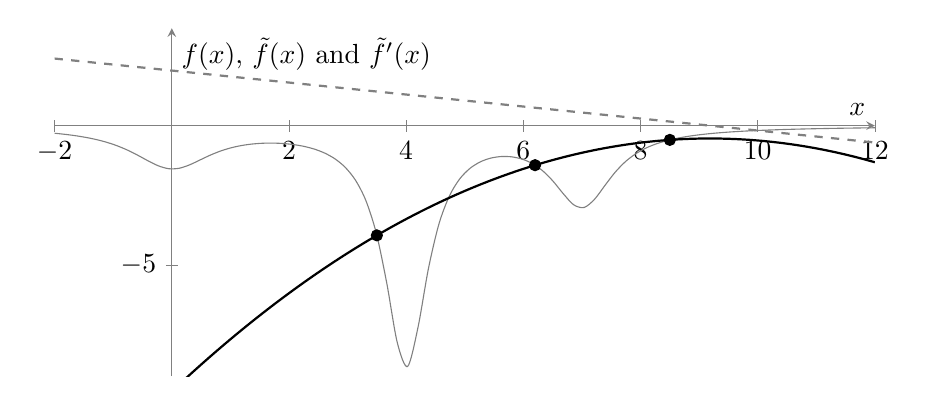
\begin{tikzpicture}
        \begin{axis}[
            width=12cm,
            height=6cm,
            axis x line=middle,
            axis y line=middle,
            xlabel={$x$},
            ylabel={$f(x)$, $\tilde{f}(x)$ and $\tilde{f}'(x)$},
            domain=-2:12,
            samples=80,
            ymin=-9, ymax=3.5,
            xmin=-2, xmax=12,
            tick style={gray},
            label style={black},
            axis line style={gray},
        ]

        \addplot[
            gray,
            thin,
            smooth,
        ] {-1/((x-0)^2 + 0.7) - 1.7/((x-4)^2 + 0.2) - 1.1/((x-7)^2 + 0.4)};
        

        \addplot[
            black,
            thick,
            smooth,
        ] {-0.10776*x^2 + 1.97913*x - 9.54881};
        
        \addplot[
            gray,
            dashed,
            thick,
            smooth,
        ] {-0.21552*x + 1.97913};
        
        \addplot[only marks, mark=*, mark size=2pt, color=black] coordinates {
            (3.5, -3.942)
            (6.2, -1.421)
            (8.5, -0.512)
        };
                
        \end{axis}
    \end{tikzpicture}
    \caption{The original Shekel function (gray thin) with a second-order approximation (solid black) fitted through three sample points (dots). The derivative of the approximation is shown as a gray dashed line. The quadratic captures the general trend but smooths out the individual foxholes.}
    \label{fig:shekel_foxholes_approximation}
\end{figure}

\newthought{Stochastic methods} add noise by approximating the loss landscape to escape local optima.
Let's approximate the 1D shekels function as a second order function by picking three points on the foxhole curve.

\newthought{The take away} is that the loss landscape is not static, but is to be engineered and formed. By approximating the loss landscape on mini-batches (different selection of points), 
we get a noisy estimate of the true loss landscape, which can help us escape local minima. The loss landscape is then of course heavily influenced by the choice of the loss function itself.
That being said, the Newton step is very sensitive to noise, we will see other approaches that deal better with this. 
\marginnote{\newthought{In deep learning,} we typically use local methods (SGD, Adam) but hope that: (1) most local minima are roughly equally good, (2) overparameterization makes bad minima rare, (3) mini-batch noise helps escape sharp minima, (4) adaptive learning rates help navigate plateaus.}







%% ---- TOPIC 2: Newton's Method for Optimization ----

\section{Newton's Method for finding Minima}
\index{Newton!optimization}


\newthought{In the hands-on,} we saw that reformulating optimization as root finding allows us to apply Newton's method to find optima:

\begin{equation}
    x_{n+1} = x_n - \frac{f'(x_n)}{f''(x_n)}.
\end{equation}

\newthought{Minima, maxima, and saddle points.} Newton's method finds points where $f''(x) = 0$, but these can be minima, maxima, or saddle points. The second derivative test distinguishes them:
\begin{enumerate}[label=(\alph*)]
    \item $f''(x^*) > 0$: local minimum (curve bends upward)
    \item $f''(x^*) < 0$: local maximum (curve bends downward)
    \item $f''(x^*) = 0$: inconclusive (possible saddle point or inflection point)
\end{enumerate}

\vspace{1.5em}
\begin{figure}[h]
    \centering
    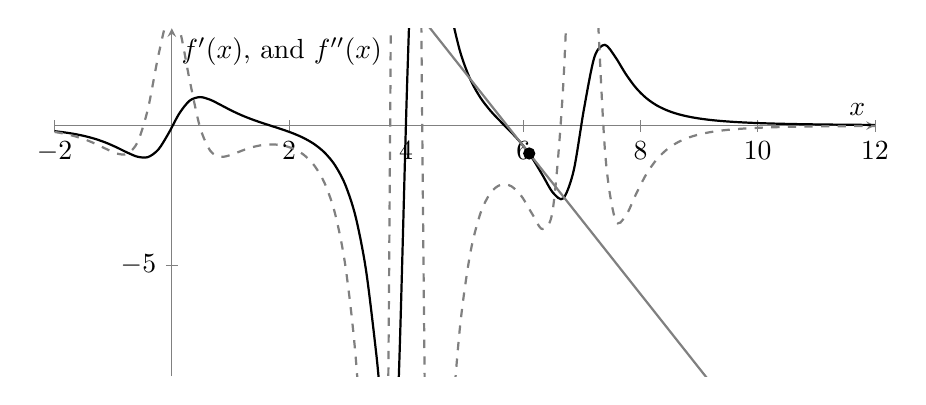
\begin{tikzpicture}
        \begin{axis}[
            width=12cm,
            height=6cm,
            axis x line=middle,
            axis y line=middle,
            xlabel={$x$},
            ylabel={$f'(x)$, and $f''(x)$},
            domain=-2:12,
            samples=80,
            ymin=-9, ymax=3.5,
            xmin=-2, xmax=12,
            tick style={gray},
            label style={black},
            axis line style={gray},
        ]
        \addplot[
            black,
            thick,
            smooth,
        ] {2*(x-0)/((x-0)^2 + 0.7)^2 + 3.4*(x-4)/((x-4)^2 + 0.2)^2 + 2.2*(x-7)/((x-7)^2 + 0.4)^2};
        
        % add a point * at 6 on the plot above
        \addplot[only marks, mark=*, mark size=2pt, color=black] coordinates {
            (6.1, -1)
        };

        \addplot[
            gray,
            dashed,
            thick,
            smooth,
        ] {2*(0.7 - 3*(x-0)^2)/((x-0)^2 + 0.7)^3 + 3.4*(0.2 - 3*(x-4)^2)/((x-4)^2 + 0.2)^3 + 2.2*(0.4 - 3*(x-7)^2)/((x-7)^2 + 0.4)^3};
                 
        \addplot[
            gray,
            thick,
        ] {-2.66*(x - 6.1) - 1};
                
        \end{axis}
    \end{tikzpicture}
    \caption{Solid black: the first derivative $f'(x)$ of the 1D Shekel function; gray dashed: the second derivative $f''(x)$. The black marker at $x=6.1$ is a sample location; the solid gray line is the tangent to $f'(x)$ at that point (slope $\approx-2.66$). The sign and magnitude of $f''(x)$ determine the Newton update direction and step size when solving $f'(x)=0$.}
    \label{fig:shekel_foxholes_derivatives_minima}
\end{figure}

\marginnote{\newthought{How would you} modify the update to find maxima instead?}
In order to direct the Newton method towards minima only, we can modify the update as such:
\begin{equation}
    x_{n+1} = x_n - \frac{f'(x_n)}{|f''(x_n)|}.
\end{equation}

In this way we ensure that we always move in the direction of decreasing $f(x)$. 
This forces the step to always move in the direction of the negative gradient (downhill so to speak).

\vspace{1.5em}
\begin{figure}[h]
    \centering
    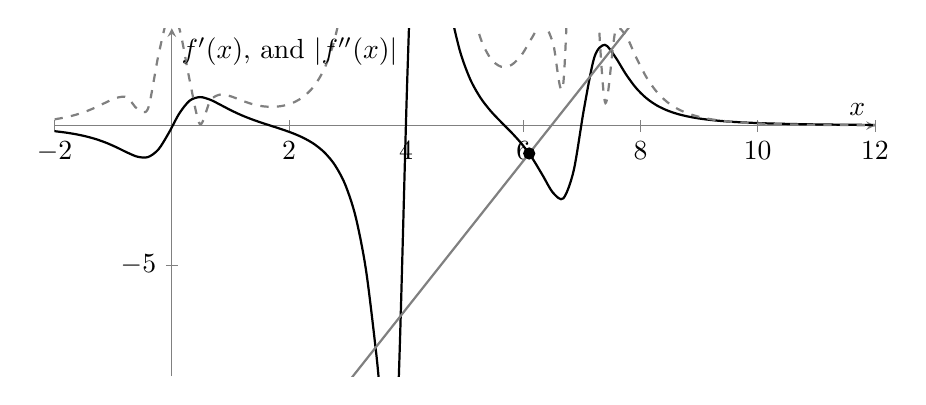
\begin{tikzpicture}
        \begin{axis}[
            width=12cm,
            height=6cm,
            axis x line=middle,
            axis y line=middle,
            xlabel={$x$},
            ylabel={$f'(x)$, and $|f''(x)|$},
            domain=-2:12,
            samples=80,
            ymin=-9, ymax=3.5,
            xmin=-2, xmax=12,
            tick style={gray},
            label style={black},
            axis line style={gray},
        ]
        \addplot[
            black,
            thick,
            smooth,
        ] {2*(x-0)/((x-0)^2 + 0.7)^2 + 3.4*(x-4)/((x-4)^2 + 0.2)^2 + 2.2*(x-7)/((x-7)^2 + 0.4)^2};
        
        \addplot[only marks, mark=*, mark size=2pt, color=black] coordinates {
            (6.1, -1)
        };

        \addplot[
            gray,
            dashed,
            thick,
            smooth,
        ] {abs(2*(0.7 - 3*(x-0)^2)/((x-0)^2 + 0.7)^3 + 3.4*(0.2 - 3*(x-4)^2)/((x-4)^2 + 0.2)^3 + 2.2*(0.4 - 3*(x-7)^2)/((x-7)^2 + 0.4)^3)};
        
        \addplot[
            gray,
            thick,
        ] {2.66*(x - 6.1) - 1};

        \end{axis}
    \end{tikzpicture}
    \caption{Solid black: the first derivative $f'(x)$; gray dashed: the absolute curvature $|f''(x)|$. Marker at $x=6.1$ shows the same sample point as above; the solid gray line illustrates replacing $f''(x)$ by $|f''(x)|$ (slope $\approx+2.66$). Using $|f''(x)|$ in the Newton denominator removes the curvature sign, enforcing downhill steps and reducing the chance of stepping toward a local maximum.}
    \label{fig:shekel_foxholes_derivatives_abs}
\end{figure}
















% ==============================================================================================
% STUDENT ACTIVATION BLOCK

\newpage
\section{Examples \& Exercises}
\index{exercises}

\marginnote{\newthought{Code} can be found at \url{https://github.com/Quillstacks/lecturecode_numericalmethods.git}.}


\newthought{Let's put the strategies to work} on concrete numbers. Suppose you are optimizing a function with 5 local minima, and the basin of attraction of the global minimum covers 15\% of the search domain ($p = 0.15$).

\marginnote{\newthought{Hint:} Use $P = 1 - (1-p)^K$ and solve for $K$: $K = \frac{\ln(1-P)}{\ln(1-p)}$.}

What is the probability of finding the global minimum with $K = 10$ random restarts?

\begin{align*}
    P &= 1 - (1 - 0.15)^{10} = 1 - 0.85^{10} \\
      &= 1 - 0.1969 = 0.803
\end{align*}

About 80\% chance, not too bad, but far from certain. How many restarts do we need for 99\%?

\begin{align*}
    K &= \frac{\ln(1 - 0.99)}{\ln(1 - 0.15)} = \frac{\ln(0.01)}{\ln(0.85)} \\
      &= \frac{-4.605}{-0.1625} \approx 28.3
\end{align*}
So $K = 29$ restarts. Now compute $K$ for $p = 0.05$ and $p = 0.01$ at the same 99\% target. 



\newthought{On your machine, } you will first design your own custom 1D Shekel function. Keep it simple in the beginning, but come back later to make it more complex.
Then first familiarize yourself with the local optimization methods you have learned so far, and apply them to your function. 
Show where Newton's method fails (again). Then explore different $x_0$ and see how the convergence behavior changes. Think again about the loss landscape and basin boundaries.
\marginnote{\newthought{Basin of Attraction.} Revisit the plots of the Shekel function, 
mark the basins of attraction for each local minimum, and estimate their relative sizes. Which one is the global minimum? 
How does this relate to the probability of finding it with random restarts?}
\marginnote{\newthought{Non-Convex Basins.} Shekel in general is non-convex, however the basins are, 
note down a function, where the basins of attraction are not so easy to map out.}

\newthought{Directing the search towards minima.} Remember the $|f''|$ trick, flips the sign of the curvature in the denominator, forcing the step to always go downhill. Think about what that means geometrically for the tangent line construction.
Then try it in code.


\newthought{Escaping Local Minima,} by global optimization strategies. Deploy random restarts and basin hopping on your custom 1D Shekel function, 
and compare how many function iterations each method needs to find the global minimum. How prone are they to getting stuck in local minima? 
How does the choice of the step size distribution affect basin hopping's performance? 

\marginnote{\newthought{Can you think of} a smart way to automatically adjust the step size distribution during optimization? 
What would be a good heuristic to follow? How could you prevent disastrous jumps? Implement it.}


\newthought{Noise and landscape engineering.} The loss landscape is not static, but is to be engineered and formed. By approximating the loss landscape on mini-batches (different selection of points),


\newthought{Code exercise:} implement random restarts and basin hopping on the 1D Shekel function.
Compare how many function evaluations each method needs to find the global minimum at $x \approx 4$.




\vspace{2em}
\newthought{Finally, let's map out the basins of attraction.} Consider the 1D Shekel function and assume a local optimizer always converges to the nearest foxhole.2

\begin{enumerate}[label=(\alph*)]
    \item Sketch (roughly) the basins of attraction for the three foxholes at $x = 0, 4, 7$. Where are the basin boundaries?
    \item If basin hopping uses a jump of $\delta \sim \text{Uniform}(-3, 3)$ starting from the local minimum $x^{\circ} = 7$,
    what is the probability that a single jump lands in the basin of the global minimum?
    \item Why might basin hopping find the global minimum faster than random restarts here?
\end{enumerate}






\section{Self-Reflection and Recap}
\index{recap}

\newthought{Self-Reflection} Questions to guide your understanding:
\begin{itemize}
    \item Why does local optimization fail on non-convex landscapes like Shekel's foxholes?
    \item How does the required effort scale withthe size of the global basin when doing random restarts?
    \item How do basin hopping differently from random restarts?
    \item What does $f''(x_n)$ tell us about the loss landscape, what does it characterize, and how can we put it to use?
    \item How does approximating the loss landscape with noisy estimates (mini-batches) help escape local optima?
    \item Choosing $x_0$ such that it lies in the basin of a local minimum, now find different ways such that your optimization method can escape it, how effective is what?
\end{itemize}

\newthought{Recap} of Key Concepts:
\begin{itemize}
    \item Local optimization methods (like Newton's method) can get stuck in local minima on non-convex functions.
    \item Global optimization strategies (random restarts, basin hopping, simulated annealing, stochasticity) are designed to explore the search space more broadly to find the global optimum.
    \item Modifying optimization methods to use curvature information $f''(x)$ allows to specify the direction of descent more accurately.
    \item The loss landscape is ours to engineer through the choice of loss function and noise, such as stochastic gradients. 
\end{itemize}


\marginnote{\newthought{Teaser.} What if we now face a high-frequency version of Shekels foxholes. What is the problem that arises?}

\newthought{Gradient descent is prone to getting stuck.} And so far our answer was merely better than brute-forcing out way out, yet again.
In the next chapter, we will learn how to smoothen loss landscape to increase the robustness of our gradient descent approach.




%%%%%%%%%%%%%%%%%%%%%%%%%%%%%%%%%%%%%%%%%%%%%%%%%%%%%%%%%%%%%%%%%%%%%%%%%%%%%%
